\chapter{Исследования}

\section{Описание исследований и расположение приёмников}

Для начала будем проводить исследования в горизонтально-слоистой среде без каких-либо аномалий. Напомню, что на рисунке \ref{fig:example} изображен срез горизонтально-слоистой среды, который мы используем в качестве решения нормального поля на первом этапе разделения полей. Далее рассмотрим горизонтально-слоистую среду с двумя аномалиями вместе, т.е для решения задачи на добавочное поле будем использовать сетку, учитывающую сразу две аномалии. После этого последовательно рассмотрим добавление в среду сначала первой аномалии потом второй, а затем сначала второй и после первой. На заключительном этапе рассмотрим временные затраты на решение задачи при использовании многоэтапной схемы разделения поля и при разбиении поля на нормальное и добавочное.

Пусть источник индукционного поля имеет радиус $R = 100$ м. от оси симметрии и имееет силу тока, равную $J_{\varphi} = 1.0$ А. Также условимся, что источник работал достаточно долго, чтобы создать стабильное электромагнитное поле. Сетка по времени: $t \in [0.0; 1.0]$ на 100 временных слоёв c начальным шагом $h_t = 10^{-5}$ с. и коэффициентом разрядки $t_k = 1.1$. После отключим наш источник, т.е. $J_{\varphi} = 0.0$ A при $t > 0.0$. Возьмём 4 приемника и расположим их вдоль линии $x = 0$ между аномалиями. Пусть они будут располагаться на расстояниях 101 м., 1000 м., 2000 м., 3000 м. от центра симметрии. На рисунке \ref{fig:receivers_info} тёмно-бирюзовой кривой нарисован индукционный источник тока, контурными линиями нарисованы положение аномальных объектов в среде, точками -- расположение приёмников.


\begin{figure}
	\centering
	\vspace*{0.7cm}
	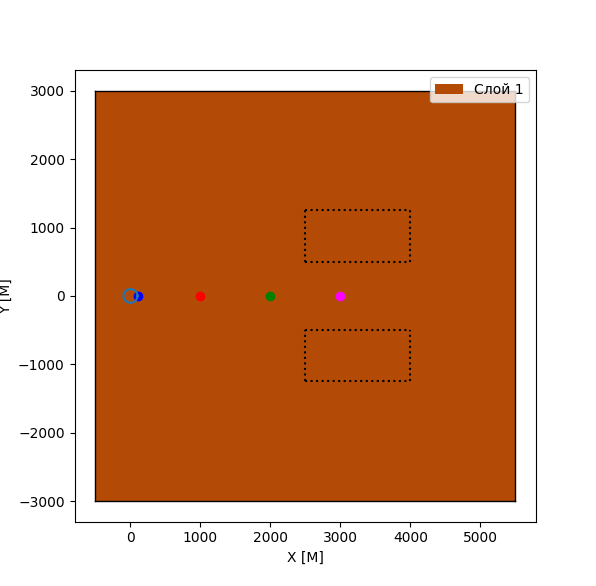
\includegraphics[width=0.7\linewidth]{images/receivers_location.png}
	\caption{Расположение приёмников}
	\label{fig:receivers_info}
\end{figure}


\section{Исследование нормального поля без аномалий}

На рисунках \ref{fig:E_phi_0} -- \ref{fig:E_phi_3} представлено распространение этого поля в среде в начальный, промежуточные и последний моменты времени. Также, проведём замеры значения напряжённости электрического поля в них. Полученные зависимости $E^0$ от времени изображены на рисунке \ref{fig:LogE}.

\begin{figure}
	\centering
	\vspace*{0.7cm}
	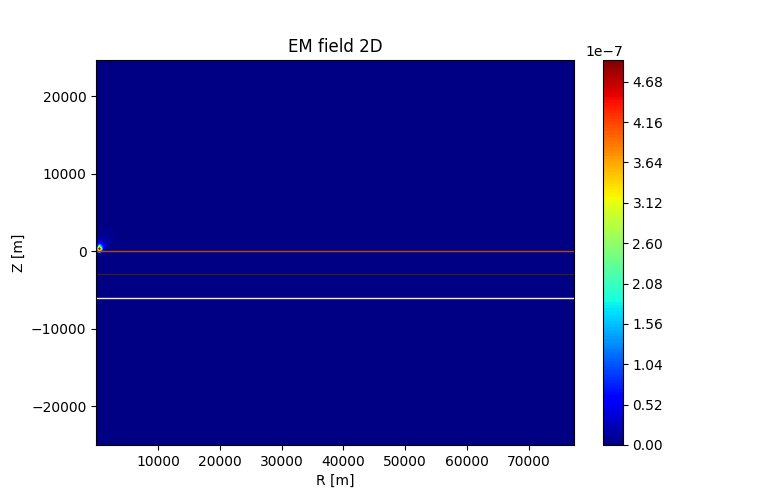
\includegraphics[width=0.95\linewidth]{images/Answer_E_time_layer_1.png}
	\caption{Решение $E_{\varphi}$ при $t = 10^{-5}$c}
	\label{fig:E_phi_0}
\end{figure}

\begin{figure}
	\centering
	\vspace*{0.7cm}
	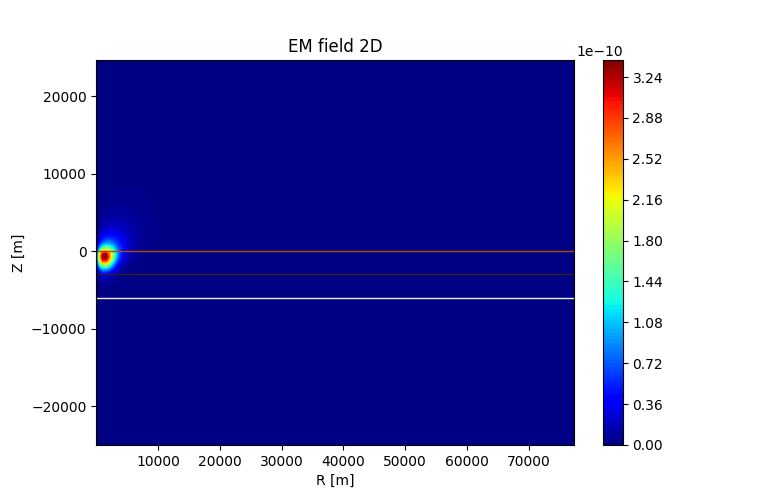
\includegraphics[width=0.95\linewidth]{images/Answer_E_time_layer_15.png}
	\caption{Решение $E_{\varphi}$ при $t = 0.01$c}
	\label{fig:E_phi_1}
\end{figure} 

\begin{figure}
	\centering
	\vspace*{0.7cm}
	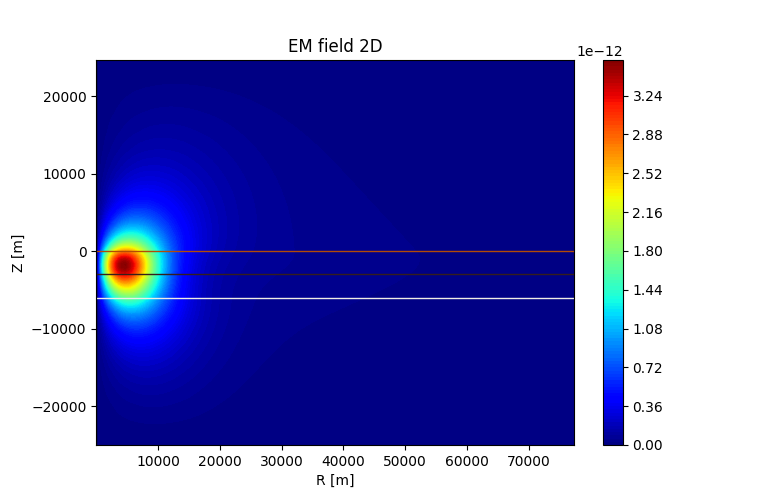
\includegraphics[width=0.95\linewidth]{images/Answer_E_time_layer_45.png}
	\caption{Решение $E_{\varphi}$ при $t = 0.1$c}
	\label{fig:E_phi_2}
\end{figure} 

\begin{figure}
	\centering
	\vspace*{0.7cm}
	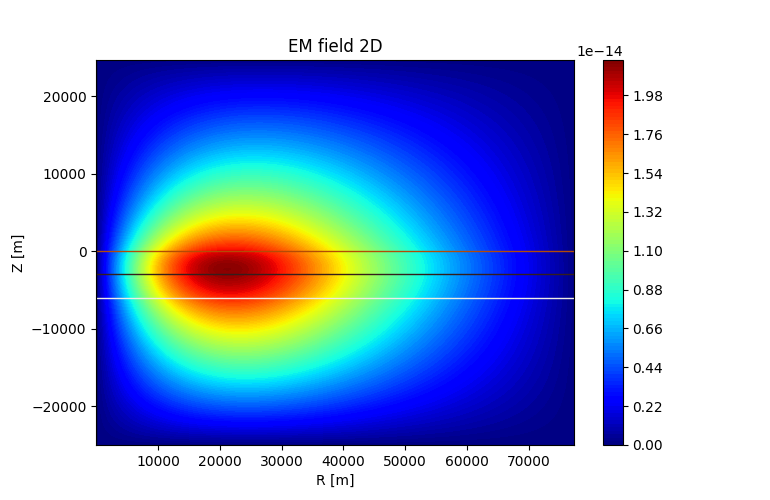
\includegraphics[width=0.95\linewidth]{images/Answer_E_time_layer_60.png}
	\caption{Решение $E_{\varphi}$ при $t = 1$c}
	\label{fig:E_phi_3}
\end{figure} 

\begin{figure}
	\centering
	\vspace*{0.7cm}
	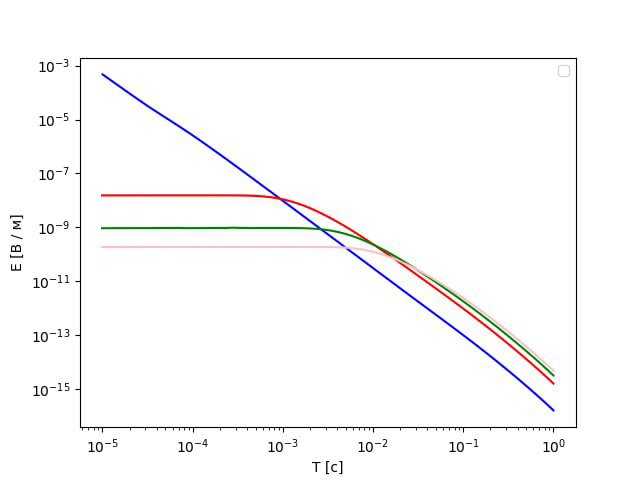
\includegraphics[width=1.0\linewidth]{images/Log_E.png}
	\caption{Зависимость значения модуля $E^0$ от времени в разных приёмниках}
	\label{fig:LogE}
\end{figure} 

Как видим, значения электрической напряжённости поля на приёмниках не имеют каких-либо резких колебаний и постепенно снижаются. Из этого можно заключить, что, как и предполагалось, никаких аномальных зон в исследуемой области нет. 

\section{Исследование в среде с двумя аномалиями}

Теперь расположим в расчётной области два аномальных объекта. Пусть первый объект имеет удельную электропроводность $\sigma_1 = 5.0$ См/м и находится в $\Omega_1 \in [2500, 4000]_x \times [500, 1250]_y \times [-2000, -750]_z$, а второй $\sigma_2 = 10.0$ См/м и находится в $\Omega_2 \in [2500, 4000]_x \times [-1250, -500]_y \times [-2000, -750]_z$. Их расположение в сечениях изображено на рисунках \ref{fig:Anomaly1} -- \ref{fig:Anomaly2}.  

\begin{figure}
	\centering
	\vspace*{0.7cm}
	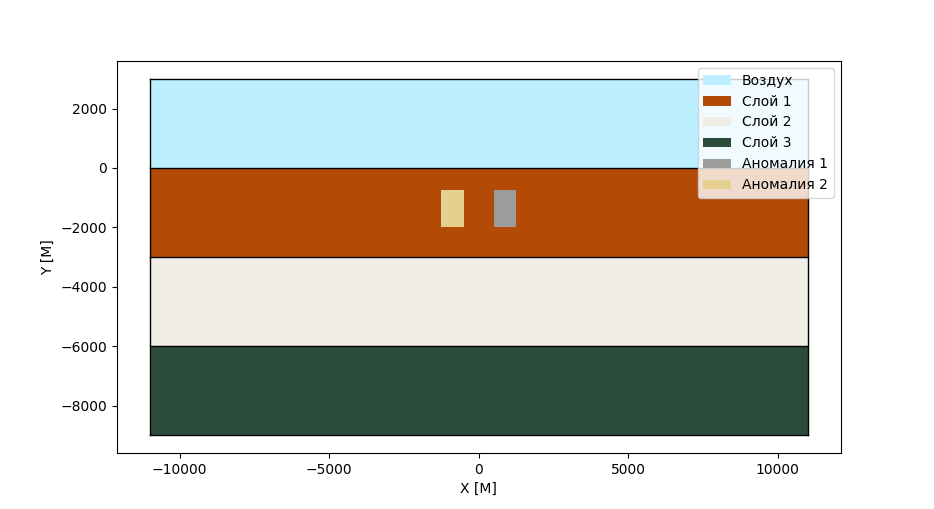
\includegraphics[width=0.8\linewidth]{images/Anomalies_1.png}
	\caption{Срез среды при $x = 2500$м}
	\label{fig:Anomaly1}
\end{figure}


\begin{figure}
	\centering
	\vspace*{0.7cm}
	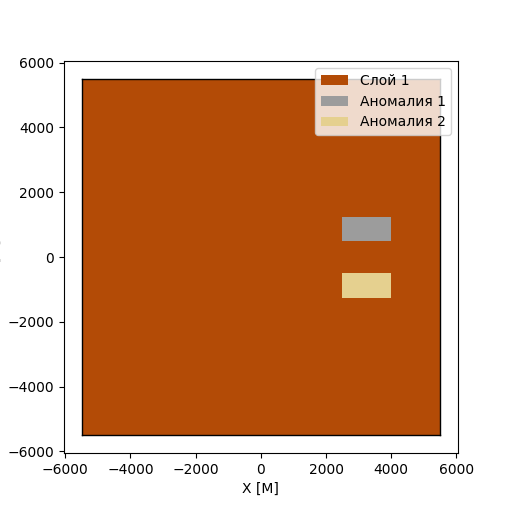
\includegraphics[width=0.7\linewidth]{images/Anomalies_2.png}
	\caption{Срез среды при $z = -1000$м}
	\label{fig:Anomaly2}
\end{figure}

Тогда графики зависимости значения напряжённости электрического поля $E$ от времени на выбранных нами приёмниках представлены на рисунке \ref{fig:LogE_both}. Процесс рассматривался с 0.002 секунды. 

\begin{figure}
	\centering
	\vspace*{0.7cm}
	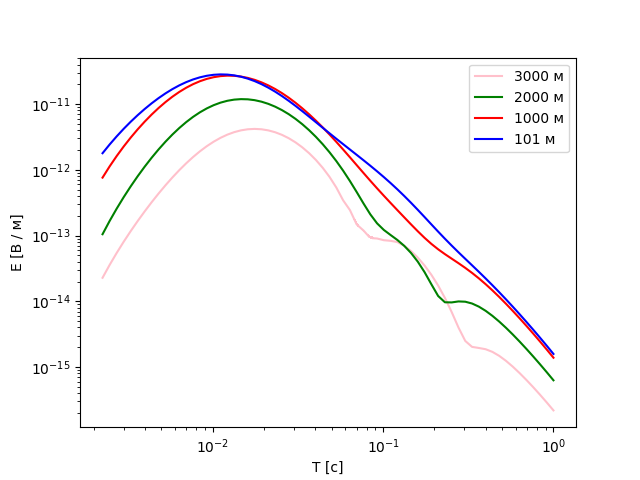
\includegraphics[width=1.0\linewidth]{images/Log_E_both.png}
	\caption{Зависимость значения модуля $E^+$ от времени в приёмниках при одновременном разделении аномалий}
	\label{fig:LogE_both}
\end{figure} 

Как можно заметить, со временем, значение модуля напряжённости электрического поля добавочных объектов сначала увеличивается, а затем уменьшается. Объяснить это можно тем, что рассеиваемое поле горизонтально-слоистой среды со временем начинает оказывать влияние на аномальный по электропроводности объект. Из-за этого модуль значения напряжённости электромагнитного поля сначала растёт, а затем плавно также рассеивается вместе с полем горизонтально-слоистой среды.

\section{Исследование многоэтапного разделения полей}

Теперь рассмотрим постепенное добавление аномальных зон в расчётную область. Пусть на первом этапе, в качестве добавочного поля будем считать поле, создаваемое объектом с удельной электропроводностью $\sigma$ = 5.0 См/м. На втором этапе в качестве нормального поля будем рассматривать поле, полученное на предыдущем этапе, а в качестве добавочного, поле создаваемое объектом с электропроводностью $\sigma$ = 10.0 См/м. Графики изменения значения напряжённости электрического поля от времени после добавления первой аномалии, а затем второй изображёны на рисунке \ref{fig:LogE_1_plus_2}.

\begin{figure}
	\centering
	\vspace*{0.7cm}
	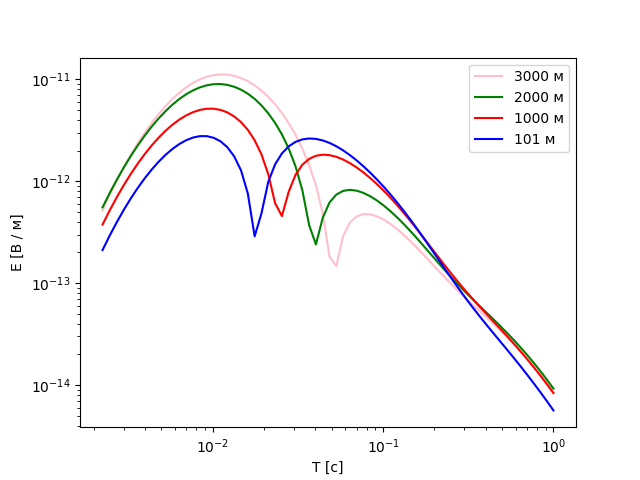
\includegraphics[width=0.75\linewidth]{images/Log_E_1_plus_2.png}
	\caption{Зависимость значения модуля $E^+$ от времени в разных приёмниках при разделении сначала первой, а затем второй аномалии}
	\label{fig:LogE_1_plus_2}
\end{figure} 


По началу значения напряжённости поля повышаются. Резкий скачок вниз можно объяснить инверсией электромагнитного поля --  направление распространения может измениться на противоположное по знаку значение.

Теперь рассмотрим постепенное добавление аномальных зон в расчётную область наоборот. На первом этапе, в качестве добавочного поля будем считать поле, создаваемое объектом с удельной электропроводностью $\sigma$ = 10.0 См/м. На втором этапе в качестве нормального поля будем рассматривать поле, полученное на предыдущем этапе, а в качестве добавочного, поле создаваемое объектом с электропроводностью $\sigma$ = 5.0 См/м. График изменения значения напряжённости электрического поля от времени после добавления первой аномалии, а затем второй изображён на рисунке \ref{fig:LogE_2_plus_1}.

\begin{figure}
	\centering
	\vspace*{0.7cm}
	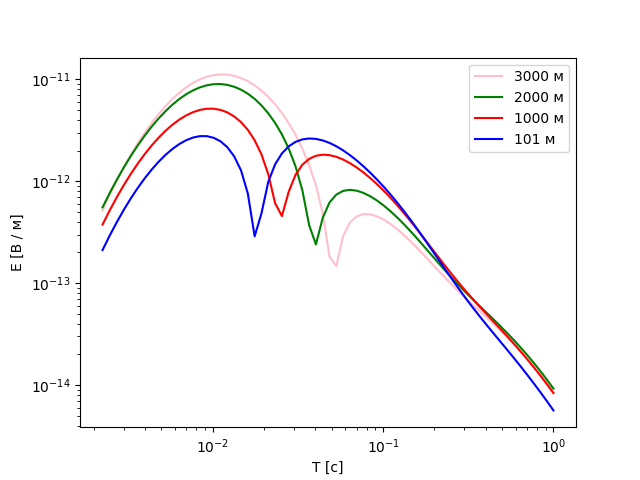
\includegraphics[width=0.75\linewidth]{images/Log_E_2_plus_1.png}
	\caption{Зависимость значения модуля $E^+$ от времени в разных приёмниках при разделении сначала второй, а затем первой аномалии}
	\label{fig:LogE_2_plus_1}
\end{figure} 

На рисунке \ref{fig:LogE_compare_1_and_2} изображено сравнение результатов первого и второго подхода к многоэтапному разделению полей. Цветными линиями показано значение напряжённости электрического поля при разделении сначала второй, а затем первой, чёрным пунктиром значение напряжённости при разделении сначала первой, а затем второй аномалий.

\begin{figure}
	\centering
	\vspace*{0.7cm}
	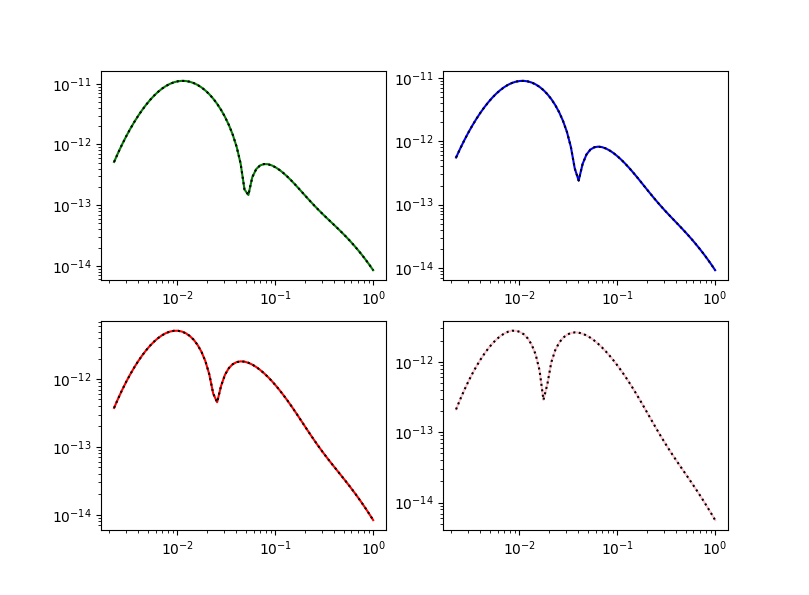
\includegraphics[width=1.0\linewidth]{images/Log_E_compare_1_and_2.png}
	\caption{Сравнение значений модуля $E^+$ от времени на разных приёмниках при разной очерёдности разделении аномалий}
	\label{fig:LogE_compare_1_and_2}
\end{figure} 


Как выяснилось, очерёдность разделения полей не дала видимых различий, следовательно результат не зависит от очерёдности добавления аномалий в расчётную область.

Поскольку очерёдность добавления аномальных объектов в расчётную область не даёт очевидной разницы, то рассмотрим на рисунке \ref{fig:LogE_compare_both_and_msrp} сравнение значений $E^+$ при одновременном разделении сразу двух объектов и при использовании многоэтапной схемы, сначала выделяя первый, а затем второй объект. Цветными линиями показаны значения при использовании многоэтапной схемы разделения полей, пунктиром при одновременном разделении сразу двух аномалий.

\begin{figure}
	\centering
	\vspace*{0.7cm}
	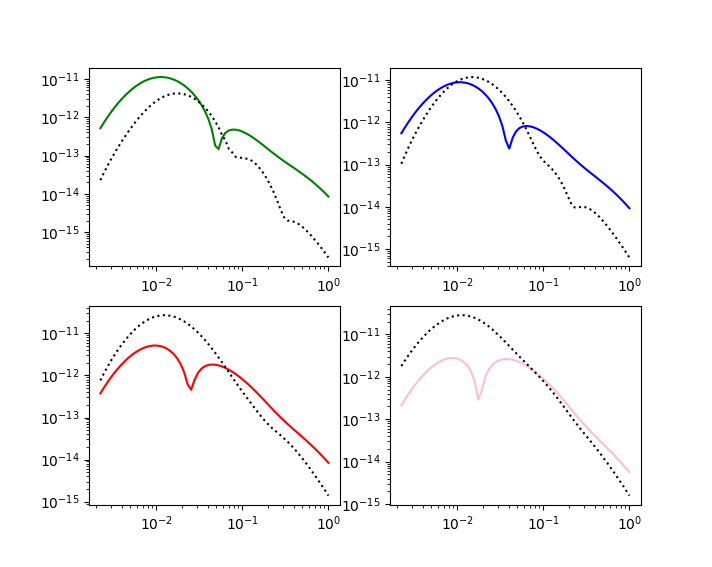
\includegraphics[width=1.0\linewidth]{images/Log_E_compare_both_with_msrp.png}
	\caption{Сравнение значений модуля $E^+$ от времени в разных приёмниках при одноэтапном и многоэтапном разделении}
	\label{fig:LogE_compare_both_and_msrp}
\end{figure}  
 

\section{Исследование явления взаимоиндукции}

Теперь предположим, что при использовании многоэтапной схемы разделения полей для обоих наших объектов можно найти, не учитывая влияния другого объекта, а учитывая лишь влияние поля в горизонтально-слоистой среде. Иными словами, значение $\overrightarrow{\textbf{E}}^n$ при учёте второй по очереди аномалии в уравнении (\ref{eq_1_6}) будет рассматриваться не суммой $E^0 + E^a$ как мы делали это прежде, а просто через $E^0$, где $E^0$ -- напряжённость электрического поля от влияния горизонтально-слоистой среды, а $E^a$ -- напряжённость электрического поля от влияния первой аномалии. На рисунках \ref{fig:LogE_isolated_1} -- \ref{fig:LogE_isolated_4} приведены сравнения значений для разных приёмников. Сплошной линией отображена зависимость при учёте напряжённости электрического поля только горизонтально-слоистой среды (то есть просто $E^0$), а пунктиром с учётом ещё и влияния другой аномалии (то есть $E^0 + E^a$).

\begin{figure}
	\centering
	\vspace*{0.7cm}
	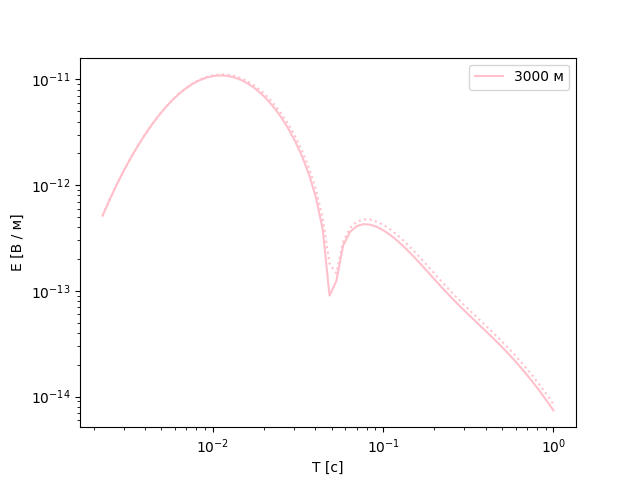
\includegraphics[width=0.7\linewidth]{images/Log_E_compare_3000.png}
	\caption{Сравнение аномалии от двух объектов с суммой аномалий от одиночных объектов на приёмнике удалённом на 3000 м}
	\label{fig:LogE_isolated_1}
\end{figure} 

\begin{figure}
	\centering
	\vspace*{0.7cm}
	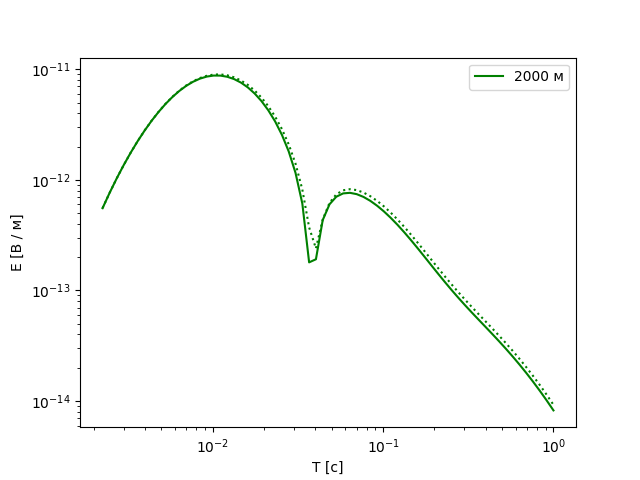
\includegraphics[width=0.7\linewidth]{images/Log_E_compare_2000.png}
	\caption{Сравнение аномалии от двух объектов с суммой аномалий от одиночных объектов на приёмнике удалённом на 2000 м}
	\label{fig:LogE_isolated_2}
\end{figure} 

\begin{figure}
	\centering
	\vspace*{0.7cm}
	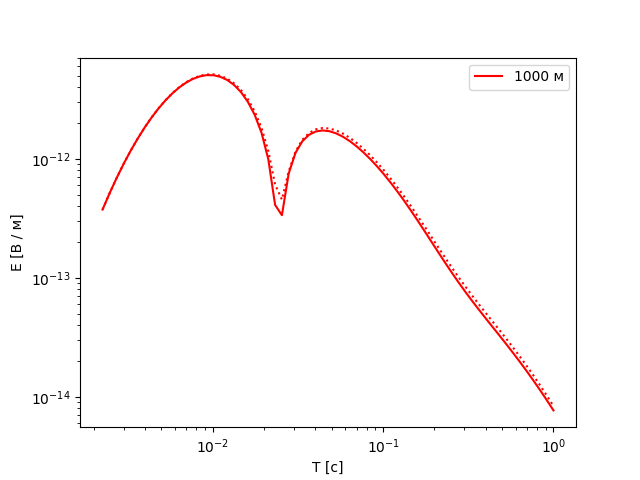
\includegraphics[width=0.7\linewidth]{images/Log_E_compare_1000.png}
	\caption{Сравнение аномалии от двух объектов с суммой аномалий от одиночных объектов на приёмнике удалённом на 1000 м}
	\label{fig:LogE_isolated_3}
\end{figure} 

\begin{figure}
	\centering
	\vspace*{0.7cm}
	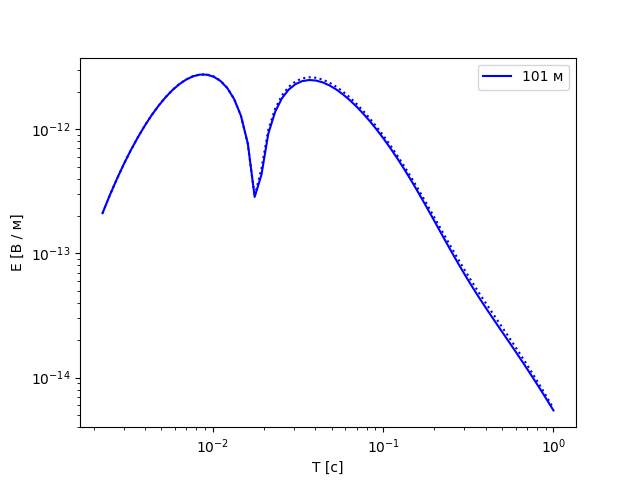
\includegraphics[width=0.7\linewidth]{images/Log_E_compare_101.png}
	\caption{Сравнение аномалии от двух объектов с суммой аномалий от одиночных объектов на приёмнике удалённом на 101 м}
	\label{fig:LogE_isolated_4}
\end{figure} 

На рисунках \ref{fig:LogE_isolated_1} -- \ref{fig:LogE_isolated_3} отчётливо видно, что пунктирная прямая, начиная примерно с 0.01 секунды, несколько выше, чем сплошная. Такую разницу можно объяснить явлением взаимоиндукции электромагнитных полей. Соответственно, такой учёт аномальных объектов при многоэтапном разделении полей не стоит применять если аномальные объекты находятся достаточно близко друг к другу.